In this section we describe the experimental results we have obtained using Cerebro and the associated tools. We conduct
tests using five sample applications. 

\begin{description}
\item[StudentInfo] A JAXRS application for managing students of a class. Provides APIs for
adding/removing students, and listing the student information.
\item[ServerHealth] An application that monitors a given web URL for server uptime. Provides an
API for obtaining the uptime statistics computed by the application.
\item[SocialMapper] A simple social networking application. Provides APIs for adding users,
comments and other resources.
\item[StockTrader] A stock trading application. Provides APIs for adding users, registering
companies, buying and selling stocks among users.
\item[Rooms] A hotel booking application. Provides APIs for registering hotels and looking up
available rooms.
\end{description}

The above applications extensively use the datastore cloud SDK interface of Google App Engine. The Rooms application
additionally uses the memcache interface.

We instrument each of the five sample applications to measure the time taken by their web APIs to execute the
enclosed code. This is done by adding some extra Java code to each of the web APIs exposed by the sample applications.
We ensure that the instrumentation does not alter the original web API code in anyway (i.e. the original algorithms, control flow
and data flow are not impacted by the instrumentation). Then for each application we also
implement a mechanism to output the measured execution times, so an external client can query and collect the execution
times of the web APIs.

We carry out each of our tests in two separate environments -- Google App Engine public cloud, and
the AppScale private cloud. The AppScale private cloud used for testing was powered by four m3.2xlarge virtual machines 
running on a private Eucalyptus cluster.

In the first set of experiments, we benchmark each application for a period of 15 to 20 hours.
During this time we run an HTTP client on a separate machine that invokes the instrumented web APIs once every minute, 
and collects the server-side execution times (as measured by the instrumentation code).
At the same time, we also run Watchtower in the same target cloud environment as the sample application being tested to
benchmark the individual cloud SDK operations. Recall that our sample applications use datastore and memcache
cloud SDK interfaces. Hence
we configure Watchtower to periodically benchmark the cloud SDK operations related to these two interfaces. 
At the end of a benchmarking run, we have two sets of data at hand:

\begin{itemize}
\item Web API execution times collected by the benchmarking HTTP client
\item Cloud SDK benchmarking data gathered by Watchtower
\end{itemize}

We now run Cerebro to make predictions regarding the web API execution time using the cloud SDK benchmarking data
collected by Watchtower. We configure Cerebro to predict an upper bound for the 95th percentile of the web API
execution time, with an upper confidence of 0.01. Cerebro generates a sequence of execution time predictions -- one 
per minute. Then we compare these predictions against the actual web API execution times measured during the same
time period. More specifically, we approximately align the sequence of predictions with the time series of actual execution
time measurements, and check whether each prediction is equal to or higher than the corresponding measurement. We consider a 
sequence of 1000 consecutive predictions and 1000 consecutive API execution
time measurements, and compute the percentage of measurements that are less than or equal to the predicted values.
 

\begin{figure}
\centering
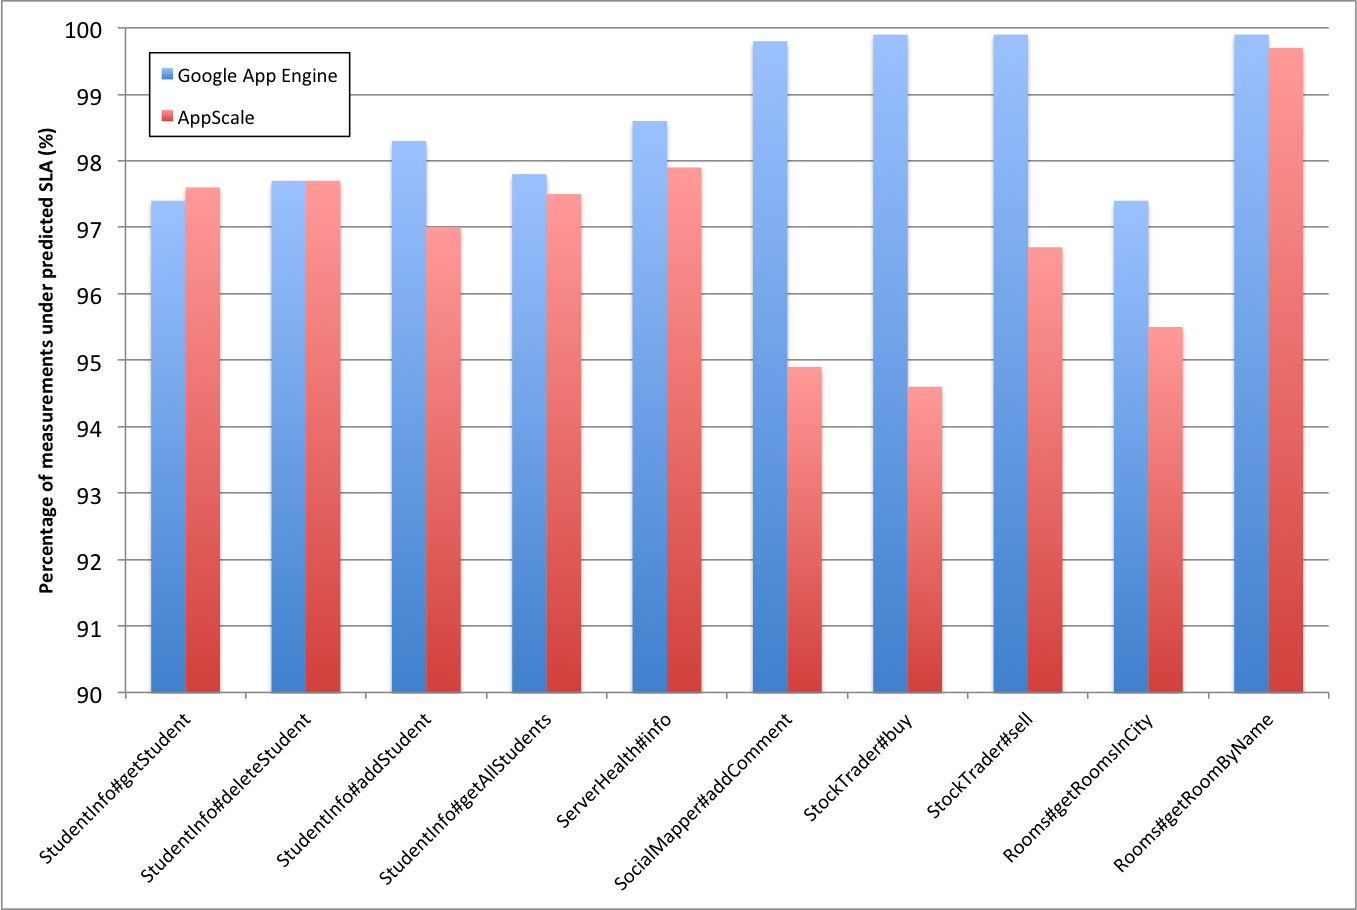
\includegraphics[scale=0.35]{accuracy_summary}
\caption{Percentage of measurements under predicted upper bound in Google App Engine and AppScale cloud platforms.}
\label{fig:accuracy_summary}
\end{figure}

Figure~\ref{fig:accuracy_summary} shows the final results of the above experiment.
Each of the columns in figure~\ref{fig:accuracy_summary} corresponds to a single web API operation in 
one of the sample applications. The columns are labeled in the form of \textit{ApplicationName\#OperationName} (a convention 
we will continue to use in the rest of the paper). To maintain clarity in the figures we do not 
illustrate the results for all web API operations in the sample applications. Instead we present the results for a selected set of 
web API operations covering all five sample applications. We note that other web API operations we tested also produce
very similar results.

Since we are using Cerebro to predict the 95th percentile of the API execution times, we expect around 95\% of the measured execution
times to be under the predicted upper bounds. According to figure~\ref{fig:accuracy_summary}, Cerebro achieves this goal for all
the cases considered in both Google App Engine and AppScale environments. The lowest percentage value observed
in our tests is 94.6\% (in the case of StockTrader\#buy on AppScale), which is also very close to the target of 95\%. Such minor
lapses below 95\% are acceptable anyway, since we expect this percentage value to be gently fluctuating around the
95\% mark over time (a phenomenon that will be illustrated in our later results). Overall, this experimental result shows us that
Cerebro produces highly accurate and reliable SLA predictions for a variety of applications running on two very
different cloud platforms.

The web API operations illustrated in figure~\ref{fig:accuracy_summary} cover a wide spectrum of scenarios that may be encountered
when statically analyzing web application code. StudentInfo\#getStudent and StudentInfo\#addStudent are by far the simplest
operations in the mix. They invoke a single cloud SDK operation each, and represent a simple datastore read scenario and a simple
datastore write scenario respectively. As per our survey on the cloud applications, these alone cover a significant portion of the 
web APIs developed for the Google App Engine and AppScale cloud platforms (1 path through the code, and 1 cloud SDK call). 
The StudentInfo\#deleteStudent operation makes two cloud SDK operations in sequence, whereas
StudentInfo\#getAllStudents performs a batch read from the datastore followed by a data dependent loop to iterate through the results.
In our experiment involving the StudentInfo\#getAllStudents operation, we had the datastore preloaded with 1000 student records, 
and Cerebro was configured to use a maximum entity count of 1000 when making predictions.

ServerHealth\#info invokes the same cloud SDK operation three times in sequence. Both StockTrader\#buy and StockTrader\#sell have
multiple paths through the code (due to branching), thus causing Cerebro to make multiple sequences of predictions -- one sequence
per path. The results shown in figure~\ref{fig:accuracy_summary} are for the longest paths which consist of seven cloud SDK invocations each. According to
our survey, 99.8\% of the execution paths found in Google App Engine applications have seven or less cloud SDK calls in them. Therefore we believe
that the web APIs in StockTrader application represent an important upper bound case. Rooms\#getRoomByName
invokes two different cloud SDK interfaces, namely datastore and memcache. Rooms\#getAllRooms is another operation that consists of
a batch read and a loop. In this case, we had the datastore preloaded with 10 entities, and Cerebro was configured to use a maximum entity
count of 10. It is indeed encouraging to see how Cerebro manages to produce highly accurate predictions for such a wide range 
of web API implementations and runtime scenarios on two cloud platforms.

\subsection{Tightness of Predictions}
In this section we discuss the tightness of the predictions generated by Cerebro. Tightness is a measure of how closely the predictions
reflect the actual response times of web APIs. This parameter is just as important as the percentage of measurements that fall under
the predicted SLA values (which 
was discussed in the previous section). Note that Cerebro can achieve a very high percentage accuracy level by simply generating a 
sequence of absurdly large predictions. But such results will obviously be of very little use to the cloud administrators and API
developers. For the predictions to be useful and even meaningful, they should be very close to the actual response times of the web APIs.

\begin{figure}
\centering
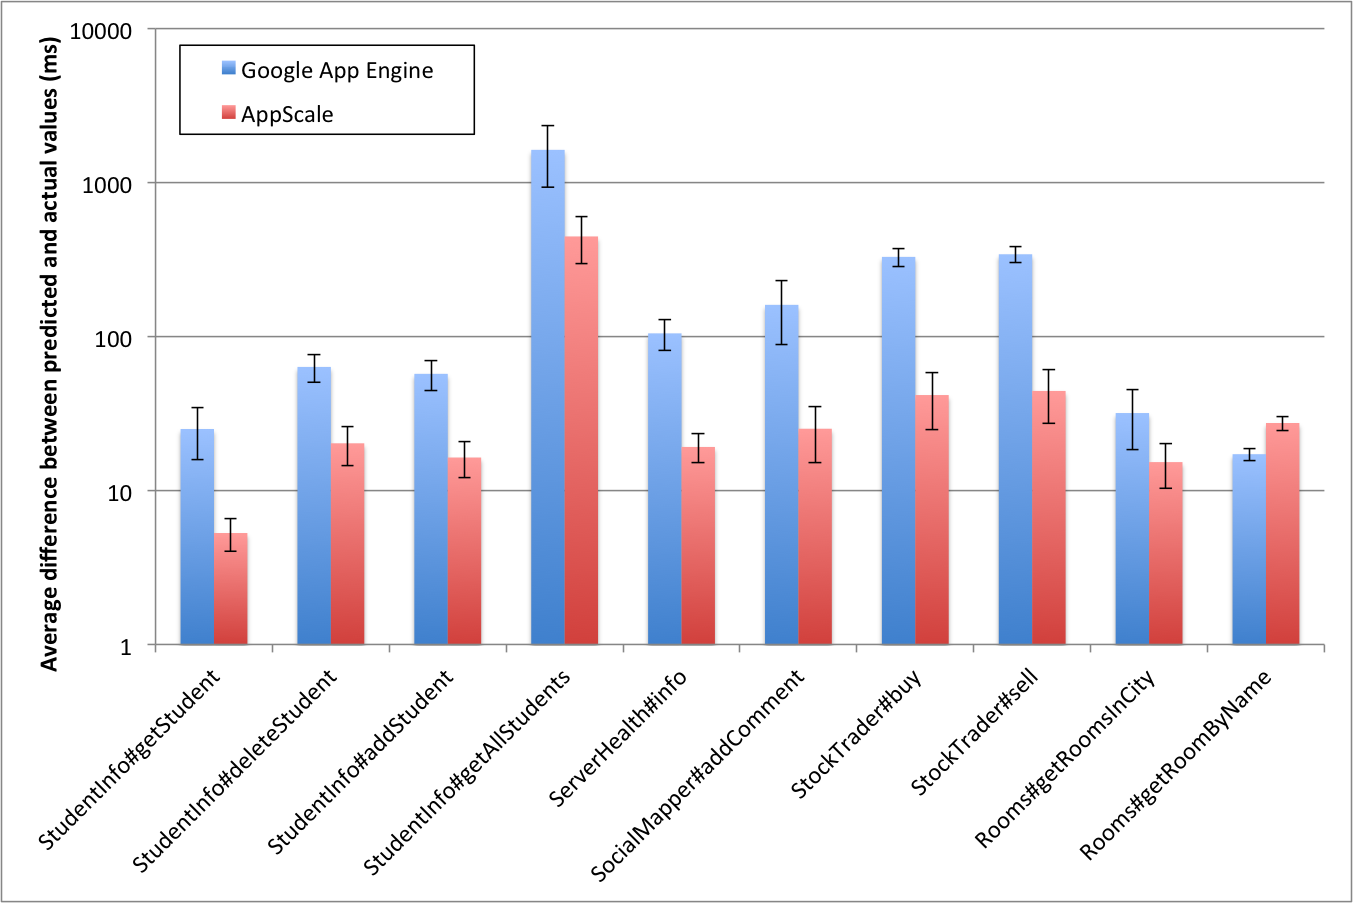
\includegraphics[scale=0.35]{diff_summary}
\caption{Average difference between predictions and actual response times in Google App Engine and AppScale. The y-axis is in log scale.}
\label{fig:diff_summary}
\end{figure}

Figure~\ref{fig:diff_summary} depicts the average difference between predicted response times and actual response times for
our sample web APIs when running in the Google App Engine and AppScale clouds. These values 
were computed considering a sequence of 1000 consecutive predictions (of 95th percentile) made by Cerebro. Within these sequences only the cases 
where the predicted value was larger than the corresponding actual execution time was taken into account. Based on our previous results
concerning the percentage accuracy, we know that this case occurs at least 95\% of the time.

According to figure~\ref{fig:diff_summary}, Cerebro generates fairly tight SLA predictions for most web API operations considered in the tests. In fact,
14 out of the 20 cases illustrated in the figure show average difference values less than 65ms. But for following scenarios Cerebro generated
predictions appear to be somewhat overly conservative:

\begin{itemize}
\item StudentInfo\#getAllStudents on both clouds
\item ServerHealth\#info, SocialMapper\#addComment, StockTrader\#buy and StockTrader\#sell on Google App Engine
\end{itemize}

To understand why Cerebro generates conservative predictions for some operations we need to 
take a closer look at the actual execution times of those operations. We take StudentInfo\#getAllStudents
operation on Google App Engine as a case study and analyze its performance characteristics in more detail. 
Note that this is the case which exhibits the largest 
average difference between predicted and actual execution times.

\begin{figure}
\centering
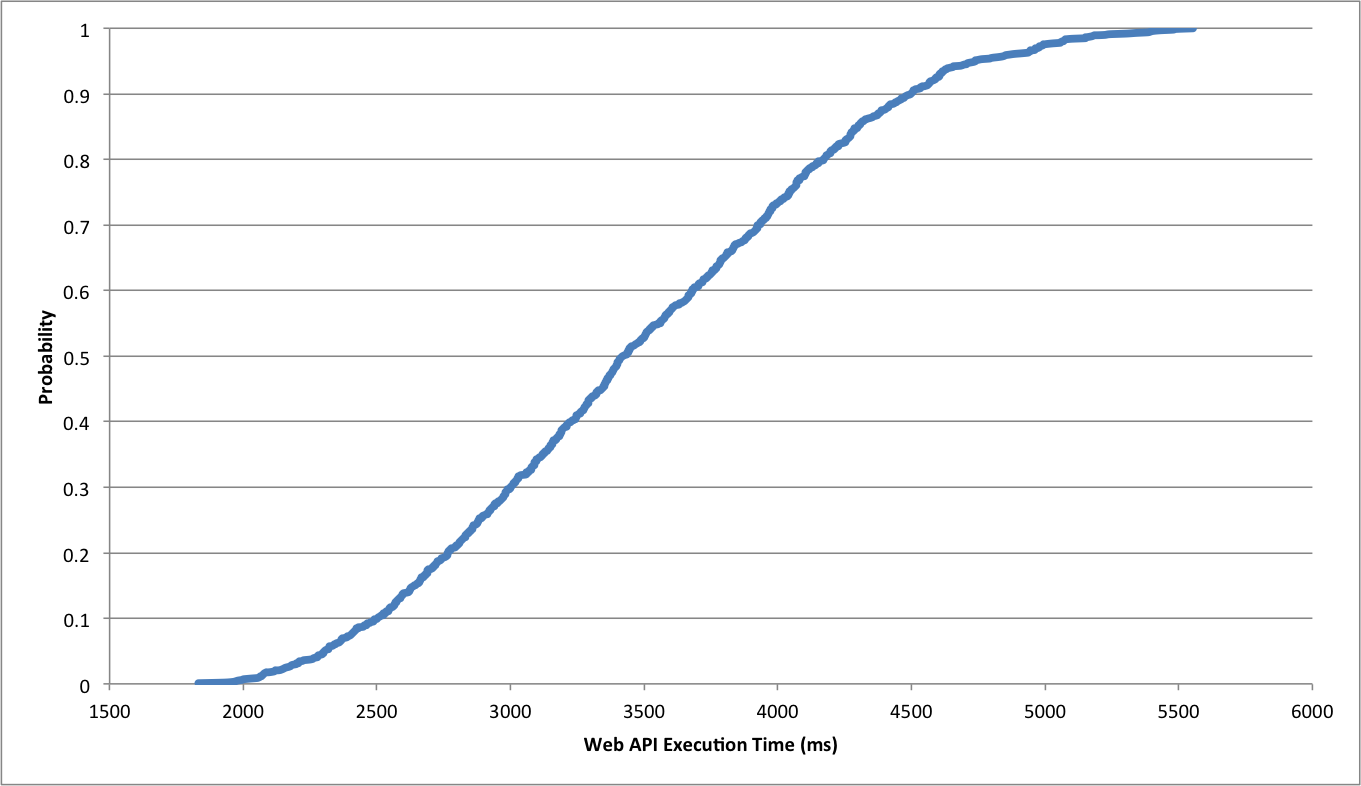
\includegraphics[scale=0.35]{get_all_students_cdf}
\caption{CDF of measured executions times of the StudentInfo\#getAllStudents operation on Google App Engine.}
\label{fig:get_all_students_cdf}
\end{figure}

Figure~\ref{fig:get_all_students_cdf} shows the CDF of measured execution times for the StudentInfo\#getAllStudents on Google
App Engine. This distribution was obtained by considering the benchmarking results gathered within a window of 1000 minutes. 
The mean and median of this distribution are 3431.79ms and 3383ms respectively. We make following two observations from the
CDF:

\begin{itemize}
\item About 50\% of the values in the distribution are higher than the mean.
\item About 10\% of the values are higher than 4500ms; more than 1000ms higher than the mean.
\end{itemize}

These two observations imply that the distribution of API execution times is significantly skewed away from the mean, and it consists
of many high outliers.
Therefore it becomes evident that StudentInfo\#getAllStudents operation results in very high execution times (i.e. high outliers) 
frequently. In order to incorporate some of these high outliers, Cerebro must be conservative and produce a large value as the prediction
of the 95th percentile. This is necessary to make sure that 95\% or more of the measurements fall under the
predicted value. However, as a consequence of this behavior the average distance between the measurements and the predictions is increased 
significantly. In retrospect even though the generated predictions are somewhat conservative, thus resulting in a high average distance 
between predictions and actual values, it is necessary in order to compensate for the variability of the web API's performance. That is, the 
less tightness in the predictions is not a limitation, but a necessary feature to ensure the correctness of the results.

Our analyses with other operations for which
Cerebro generates conservative bounds have also shown similar results. That is, when the performance of the web API is highly variable and contains
many high outliers, Cerebro predictions become less tight. In other words, Cerebro trades off tightness of the predictions for their accuracy.

\begin{figure}
\centering
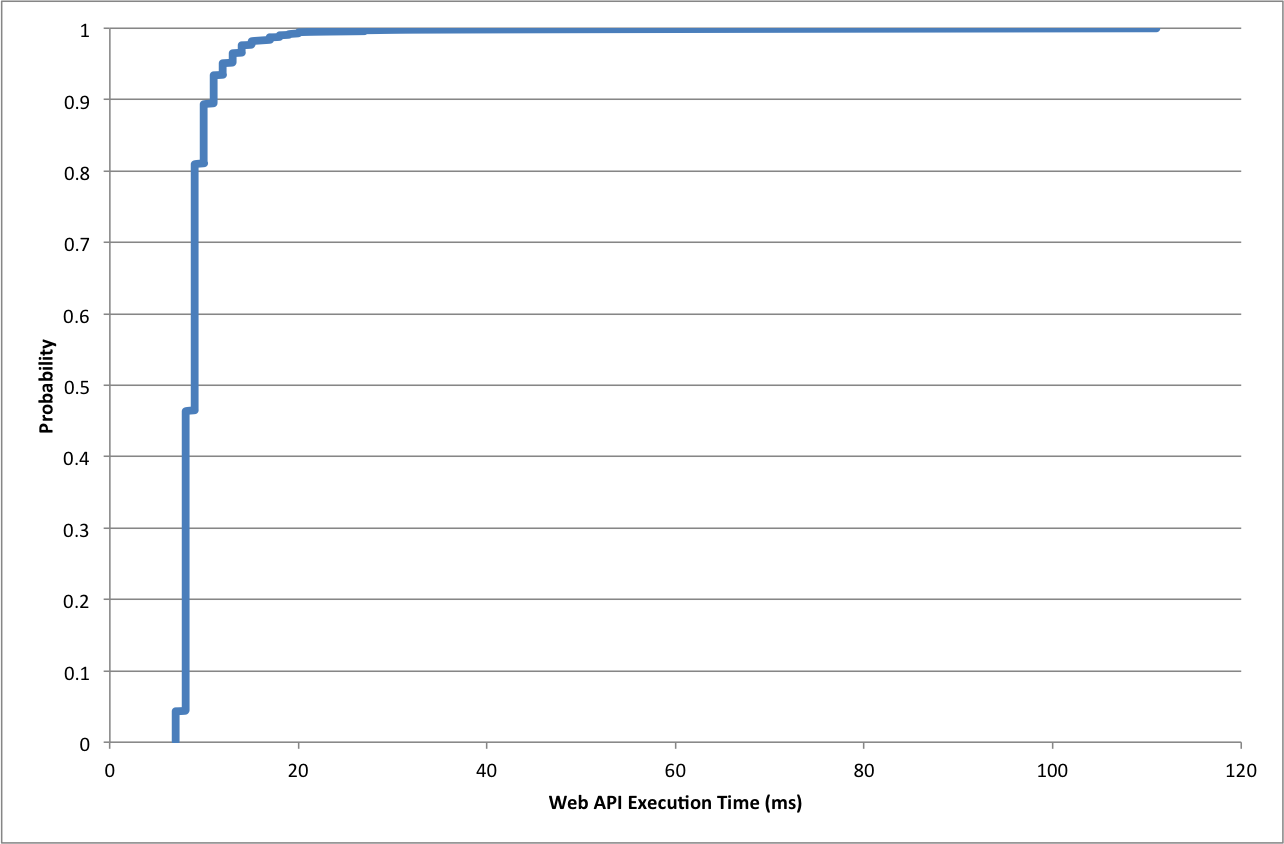
\includegraphics[scale=0.35]{get_student_cdf}
\caption{CDF of measured executions times of the StudentInfo\#getStudent operation on AppScale.}
\label{fig:get_student_cdf}
\end{figure}

To further reinforce this conclusion, we also take a close look at one of the web API operations that result in very tight predictions. 
Figure~\ref{fig:get_student_cdf} shows the CDF of the measured execution times for the StudentInfo\#getStudent operation on
AppScale cloud. Again we are considering a time frame of 1000 minutes to obtain this graph.
This particular distribution has a mean of 9.19 and a median of 9. Given that only 19\% of the values are larger than the mean, 
and only 2\% of the values are larger than 18ms (twice the mean), 
we can conclude that this distribution is much more stable and have very few high outliers. This enables Cerebro to generate much
tighter predictions, without compromising the accuracy of the results. Based on these results we can conclude that Cerebro produces
very tight upper bound predictions for web APIs whose performance is more stable over time. For APIs with highly variable performance
traits resulting in many high outliers, Cerebro generates more conservative and less tight predictions.

The reason why AppScale's performance is so stable over time is because it's a private cloud platform, deployed on a set of closely controlled 
and monitored cluster of VMs. We have total control
over how much resources are assigned to these VMs, and we ensure that they run in total isolation from the other processes running on the underlying hardware.
This is never the case when running our sample applications on Google App Engine, where we have no control over the underlying VMs, hardware and the
scheduling mechanism. Another related, but interesting outcome of these results is that large-scale public cloud platforms like Google App Engine, while
highly scalable, may not be able to support tight performance SLAs. Their performance is subject to high variations making it difficult to always support attractive
performance guarantees. Small private cloud platforms on the other hand can provide much better, consistent and stable performance guarantees, albeit their
poor scalability. From an organization's point of view this could be a strong motivator to adopt private cloud over public clouds.

\subsection{Prediction Accuracy Over Time}

\begin{figure}
\centering
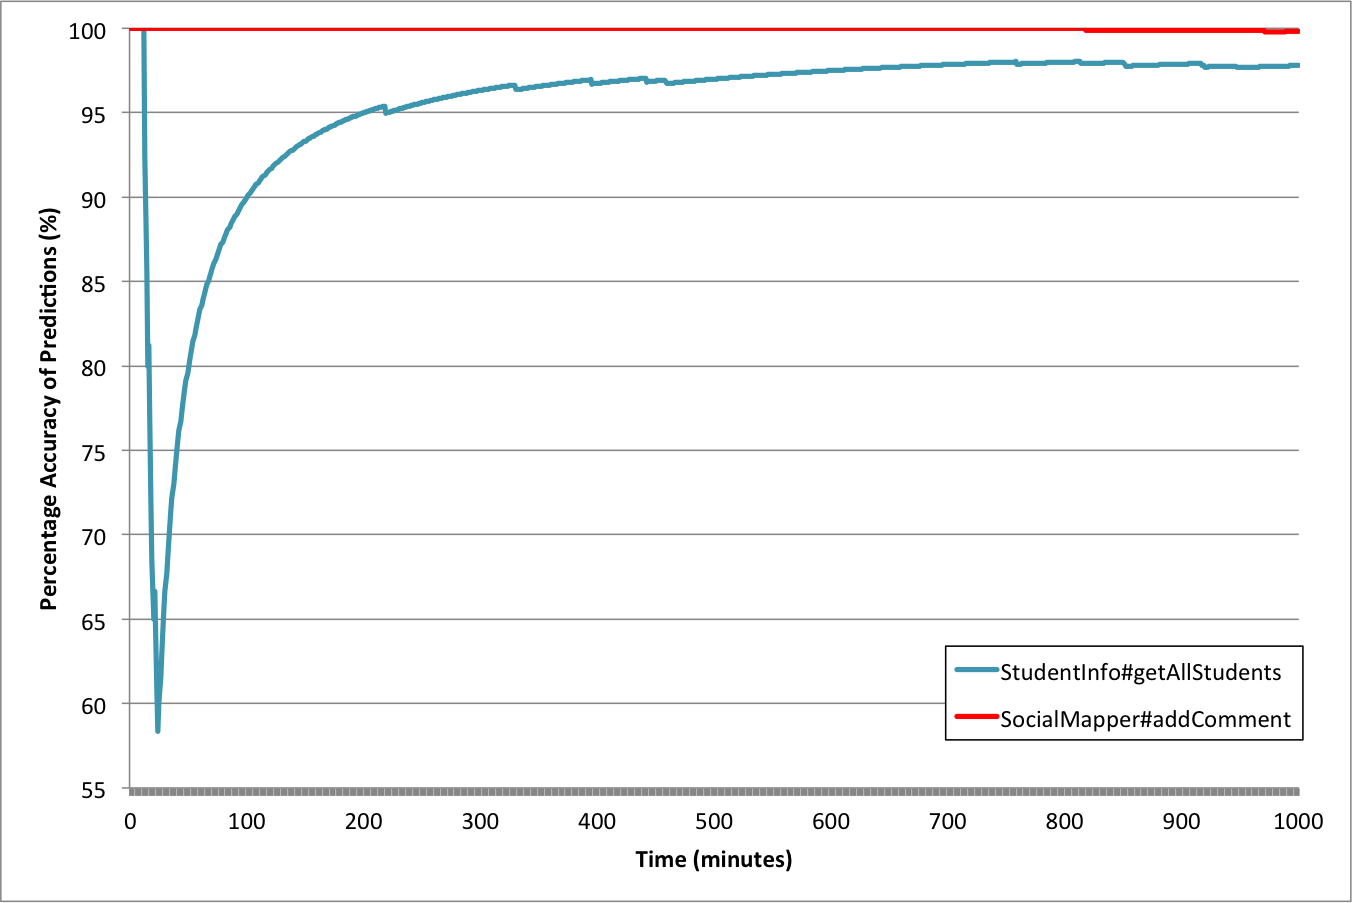
\includegraphics[scale=0.35]{gae_accuracy}
\caption{Percentage accuracy of predictions made on Google App Engine.}
\label{fig:gae_accuracy}
\end{figure}

\begin{figure}
\centering
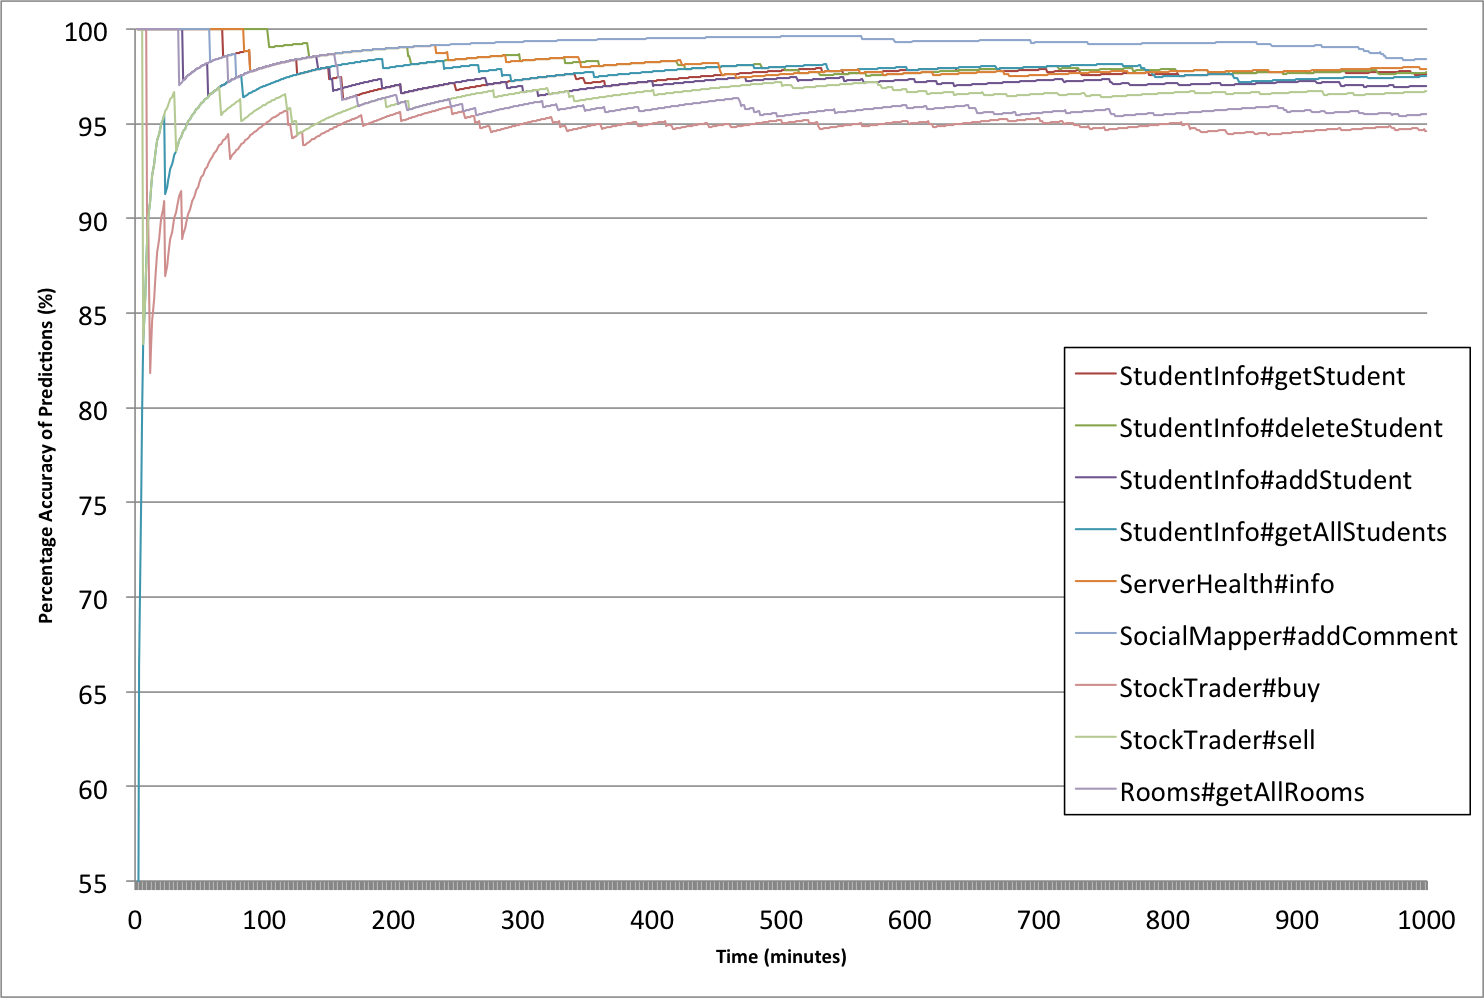
\includegraphics[scale=0.35]{as_accuracy}
\caption{Percentage accuracy of predictions made on AppScale.}
\label{fig:as_accuracy}
\end{figure}

Figure~\ref{fig:gae_accuracy} shows the percentage accuracy of the Cerebro predictions made in the Google App Engine 
public cloud environment. Each of the curves correspond to a single web API operation in one of the sample applications. 
The curves are labeled in the form of \textit{ApplicationName\#OperationName} (a convention we will continue to use
in the rest of the paper). To maintain clarity in the figures we do not 
illustrate the results for all web API operations in the sample applications. Instead we present the results for a selected set of 
web API operations covering all five sample applications. We note that other web API operations we tested also produce
very similar results.

As expected QBETS takes some time to learn
from the time series data captured by Watchtower. This is when we see large fluctuations in the percentage accuracy. But
once QBETS has converged it consistently produces highly accurate predictions regarding the 95th percentile of the web API
response time. In the worst case QBETS takes up to 200 minutes to converge. This is the case with the
StudentInfo\#getAllStudents operation. After 275 minutes, we see highly accurate predictions being made on all web API
operations considered in the tests. After this point, we consistently see percentage accuracy values higher than 96\%. Note that
we had configured Cerebro to predict the 95th percentile of the web API executions time. Therefore as long as Cerebro produces
results with a percentage accuracy close to or higher than 95\%, we can consider the predictions to be correct and reliable.

Figure 2 shows the same results calculated by running the sample applications and the Watchtower in the AppScale private cloud
environment. [More content to Follow -- some experiments still in progress]